To assess LSTM performance outside of the EVER data, a time series was simulated from an ARIMA model \citep{cowpertwait2009introductory}, given by
$$\Delta X_t = 3\cdot X_{t-1} + 0.9\cdot \varepsilon_t$$
$$\Delta X_t = X_t - X_{t-1}$$
For the data simulated from the ARIMA model, the architecture seen in Table \ref{tab:ARIMAArchitecture} was chosen through Bayesian Optimization \citep{snoek2012practical}. The architecture was chosen to have 3 LSTM layers with number of nodes ranging from 8 to 64 and dropout rates of either 0.01, 0.05, 0.1, or 0.15.This model was trained for 12,000 iterations, resulting in the point predictions seen in Figure \ref{fig:ARIMATraining} for 120 `days' out of the training data. The LSTM predictions appear to have poor initial performance but begin to capture some of the sinosoidal nature of the data after 10,000 iterations.
\begin{table}[hbt!]
\centering
\begin{tabular}{|c|c|c|c|}
    \hline 
    Layer & \# Nodes & Act F'n & Dropout Rate \\
    \hline
    LSTM & 8 nodes & Tanh  & .01  \\
    \hline
    LSTM & 15 nodes & Tanh & .05\\
    \hline
    LSTM & 39 nodes & Tanh & .15\\
    \hline
\end{tabular}
\caption{A table depicting the architecture of the LSTM trained on the simulated ARIMA data.}
\label{tab:ARIMAArchitecture}
\end{table}

\begin{figure}[hbt!]
    \centering
    \subfloat[2,000]{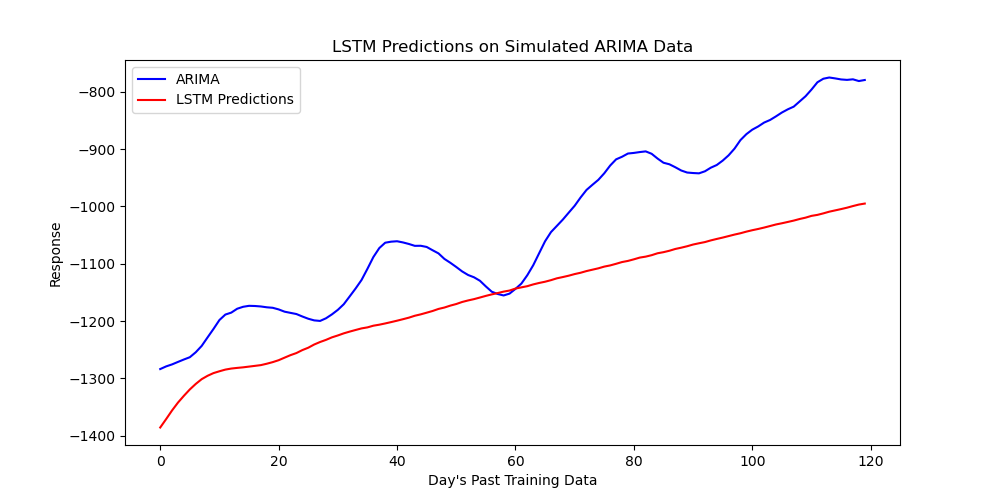
\includegraphics[width=0.5\linewidth]{"Figures/Model Diagnostics/ARIMA_model_1.png"}}
    \subfloat[4,000]{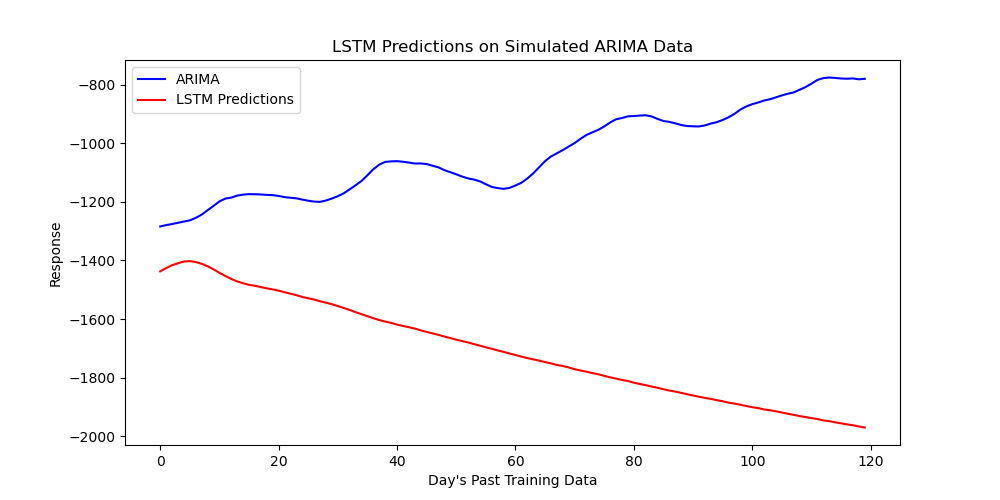
\includegraphics[width=0.5\linewidth]{"Figures/Model Diagnostics/ARIMA_model_3.png"}}\\
    \subfloat[6,000]{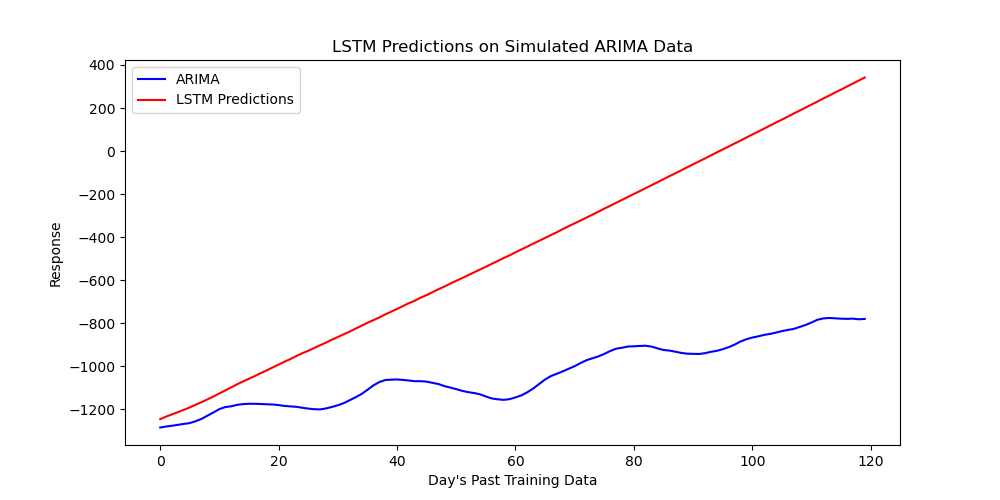
\includegraphics[width = 0.5\linewidth]{"Figures/Model Diagnostics/ARIMA_model_5.png"}}
    \subfloat[8,000]{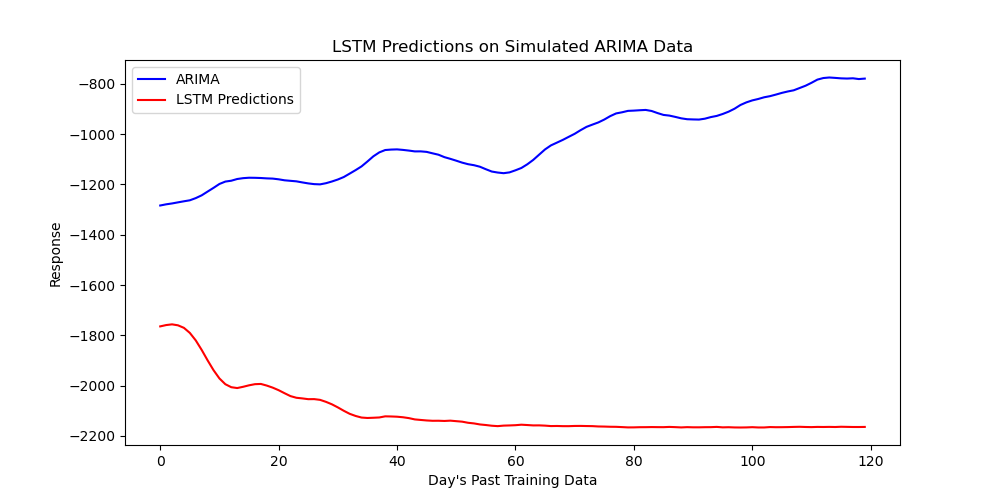
\includegraphics[width = 0.5\linewidth]{"Figures/Model Diagnostics/ARIMA_model_7.png"}}\\
    \subfloat[10,000]{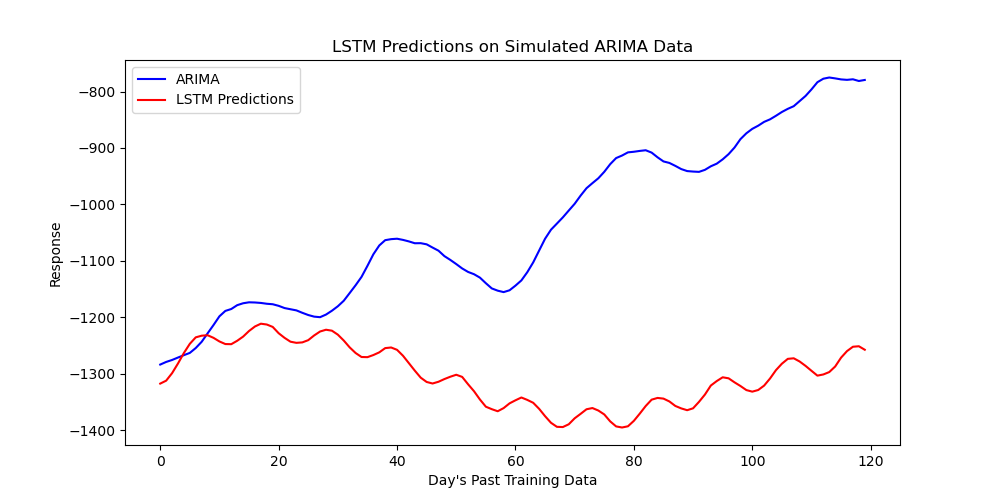
\includegraphics[width=0.5\linewidth]{"Figures/Model Diagnostics/ARIMA_model_9.png"}}
    \subfloat[12,000]{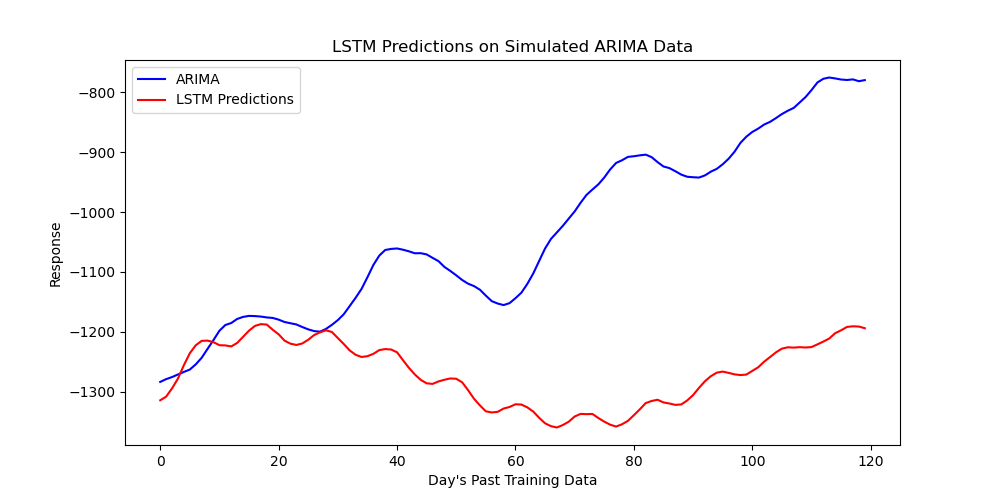
\includegraphics[width=0.5\linewidth]{"Figures/Model Diagnostics/ARIMA_model_11.png"}}
    \caption{A plot showing the LSTM predictions during the training process on the ARIMA simulated data.}
    \label{fig:ARIMATraining}
\end{figure}
\FloatBarrier

\FloatBarrier
